\section{Introduction and Goals}

According to the \acrfull{fao} in 2019 931 millions tonne of food were wasted \cite{refart:FAOFW}. This has
environmental, but special social consequences. In a world where approximately 9.9\% of the \cite{refart:AAHWH}
population suffers from hunger that waste percentage sounds paradoxal.

According to \acrfull{un} 5\% of the global food loss and waste comes from restaurants \cite{refart:UNSP}. 
The solution for this problem must be locally applied so its effects can be seen in a global structure. To do 
so we propose to develop a mobile application that connects restaurants, bakeries and or pastries to clients. The
former would offer their remaining products, which are still consumable, prior to the closing time, to a small price
and the latter would browser in the app to find which shops are offering products. 

We as ``Clean Up the World \textregistered'' are a rising StartUp whose main concerns is to find environmental solutions to
daily problems. Our portfolio includes projects about management of waste and optimization of household water 
usage. This product we want to develop targets small communities, like small cities or regions within a big city, 
to reduce the amount of wasted consumable food.

With our project we want to achieve the following goals:

\begin{itemize}
    \item Connect \glsplural{provider} with \glsplural{client}, so the former can offer products that the latter
    can purchase
    \item Collect statistical data about waste reduction within the \glsplural{provider}
    \item Promote reduction of food waste that still could be consumed
    \item Allow \glsplural{client} to have a different dining experience.
    \item Allow \glsplural{provider} to promote their products and gather new clients.
\end{itemize}

\subsection{Design Purpose}

The main purpose of this architecture is creating exploratory prototype of an \gls{app}. We aim to test it with potential 
\gls{stakeholder} and regions to analyze their general acceptance and wishes \cite{refbook:DSHC} and get a fast feedback. 

This prototype will also make it feasible to identify unknown needs an wishes of the potential \gls{stakeholder}, so we 
can eventually increase the scope of functionality. Exploring this domain will also provide us with information regarding 
the behavior of our \gls{stakeholder} when it comes to buying and serving food that would be wasted, but is still consumable.

\subsection{Requirement Overview} \label{Requirement_Overview}

The following functionalities should provide a brief description of the main requirements of the app:

\begin{table}[H]
    \setstretch{1.0}
    \begin{tabularx}{\textwidth}{llX}
    \toprule
    Id & Requirement & Description  \\
    \midrule
    F-1 & Register as \gls{client}. & A \gls{client} can register to the app with its e-mail.\\
    F-2 & Login & After registration \gls{client} can login into the app. \\
    F-3 & Purchase option & A registered \gls{client} can purchase an available offer (see F7).\\
    F-4 & Filter/search options & A \gls{client} can perform filter and search actions for products.\\
    F-5 & Register as \gls{provider} & A \gls{provider} can register with store and add logos and picutres.\\
    F-6 & Create offer & A registered \gls{provider} can publishes what products they are offering with price 
    and ammount. \\
    F-7 & Upload offer & A registered \gls{provider} can add, edit or remove offers to his catalog.\\
    F-8 & Check orders & A registered \gls{provider} can check all existing orders.\\
    \bottomrule
    \end{tabularx}
\end{table}

\newpage
The following \gls{use case diagram} displays an overview of the primary functionality of the app:

\begin{figure}[H]
    \centering
    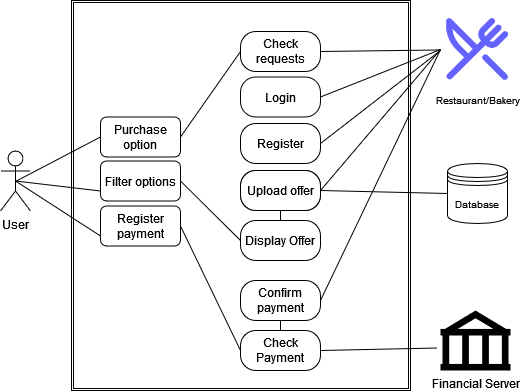
\includegraphics[width=0.7\textwidth]{assets/preliminary_use_case.png}
    \caption{Preliminary functions}
    \label{fig:preliminary_use_case}
\end{figure}

\subsection{Qualitiy Goals}

The key qualities of this app are described in the table below:

\begin{table}[H]
    \setstretch{1.0}
    \begin{tabularx}{\textwidth}{|c|c|X|}
        \toprule
        \multicolumn{1}{c}{Quality} & \multicolumn{1}{c}{Priority} & \multicolumn{1}{c}{Motivation} \\
        \midrule
        \textbf{Usability} & 1 & The app allows users to perform login, purchase and uploads within maximum 3 
        steps or page changes. Each step or page contains no more than 140 characters of instruction. \\
        \textbf{Interoperability} & 2 & The app allows registration and payment using credentials of other platforms
        (i.g \gls{mobile payment gateway} and \gls{federated login}). \\
        \textbf{Performance} & 3 & The app responds to user's interaction within few seconds. \\
        \bottomrule
    \end{tabularx}
\end{table}

\subsection{Stakeholders} 

The main \glsplural{stakeholder} of this app are described in the table below:

\begin{table}[H]
    \setstretch{1.0}
    \begin{tabularx}{\textwidth}{lX}
    \toprule
    Stakehoder & Description   \\
    \midrule
    Providers & Owner of a restaurant, bakery or pastry. \\
    Clients & Person who wants to buy last minute products from a provider. \\
    Developers & Team in charge of creating the application using existing tactics and creating new solutions. \\
    Boarding Committee of \\ ``Clean Up the Word (R)'' & Members of the management team who wants to delivery 
    environmental solution do daily problems \\
    Environment Activist & Part of the society who aims to find environmental solutions to daily problems. \\
    \bottomrule
    \end{tabularx}
\end{table}